\documentclass{standalone}
\usepackage{tikz}
\usetikzlibrary{patterns, positioning}

\begin{document}
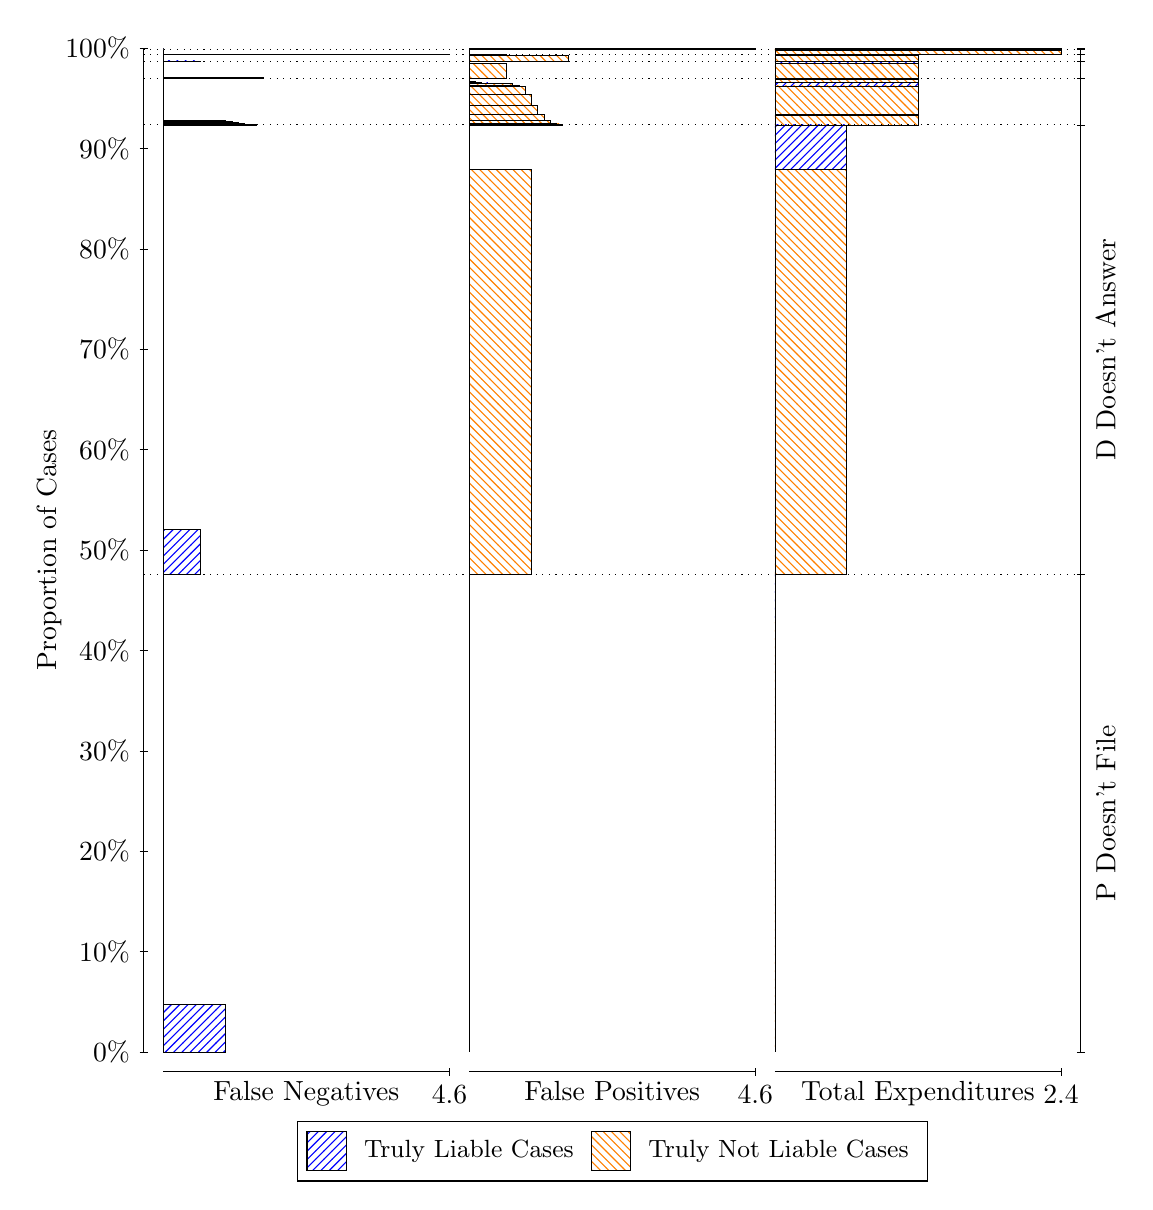
\begin{tikzpicture}
\draw[black, very thin] (1.5,1.75) -- (1.5,14.5);
\node[rotate=90, anchor=center] at (0.3, 8.125) {Proportion of Cases};
\draw[black, very thin] (1.45,1.75) -- (1.55,1.75);
\node[anchor=east] at (1.45, 1.75) {0\%};
\draw[black, very thin] (1.45,3.025) -- (1.55,3.025);
\node[anchor=east] at (1.45, 3.025) {10\%};
\draw[black, very thin] (1.45,4.3) -- (1.55,4.3);
\node[anchor=east] at (1.45, 4.3) {20\%};
\draw[black, very thin] (1.45,5.575) -- (1.55,5.575);
\node[anchor=east] at (1.45, 5.575) {30\%};
\draw[black, very thin] (1.45,6.85) -- (1.55,6.85);
\node[anchor=east] at (1.45, 6.85) {40\%};
\draw[black, very thin] (1.45,8.125) -- (1.55,8.125);
\node[anchor=east] at (1.45, 8.125) {50\%};
\draw[black, very thin] (1.45,9.4) -- (1.55,9.4);
\node[anchor=east] at (1.45, 9.4) {60\%};
\draw[black, very thin] (1.45,10.675) -- (1.55,10.675);
\node[anchor=east] at (1.45, 10.675) {70\%};
\draw[black, very thin] (1.45,11.95) -- (1.55,11.95);
\node[anchor=east] at (1.45, 11.95) {80\%};
\draw[black, very thin] (1.45,13.225) -- (1.55,13.225);
\node[anchor=east] at (1.45, 13.225) {90\%};
\draw[black, very thin] (1.45,14.5) -- (1.55,14.5);
\node[anchor=east] at (1.45, 14.5) {100\%};

\draw[black, very thin] (13.4,1.75) -- (13.4,14.5);
\draw[black, very thin] (13.35,1.75) -- (13.45,1.75);
\node[anchor=west] at (13.35, 1.75) {};
\draw[black, very thin] (13.35,7.8154) -- (13.45,7.8154);
\node[anchor=west] at (13.35, 7.8154) {};
\draw[black, very thin] (13.35,13.524) -- (13.45,13.524);
\node[anchor=west] at (13.35, 13.524) {};
\draw[black, very thin] (13.35,14.11) -- (13.45,14.11);
\node[anchor=west] at (13.35, 14.11) {};
\draw[black, very thin] (13.35,14.327) -- (13.45,14.327);
\node[anchor=west] at (13.35, 14.327) {};
\draw[black, very thin] (13.35,14.422) -- (13.45,14.422);
\node[anchor=west] at (13.35, 14.422) {};
\draw[black, very thin] (13.35,14.479) -- (13.45,14.479);
\node[anchor=west] at (13.35, 14.479) {};
\draw[black, very thin] (13.35,14.5) -- (13.45,14.5);
\node[anchor=west] at (13.35, 14.5) {};

\draw[black, very thin, pattern color=blue, pattern=north east lines] (1.75,1.75) rectangle (2.5399,2.3565);
\draw[black, very thin, pattern color=orange, pattern=north west lines] (1.75,2.3565) rectangle (1.75,7.8154);
\draw[black, very thin, pattern color=blue, pattern=north east lines] (1.75,7.8154) rectangle (2.2239,8.386);
\draw[black, very thin, pattern color=orange, pattern=north west lines] (1.75,8.386) rectangle (1.75,13.524);
\draw[black, very thin, pattern color=blue, pattern=north east lines] (1.75,13.524) rectangle (2.9348,13.527);
\draw[black, very thin, pattern color=blue, pattern=north east lines] (1.75,13.527) rectangle (2.8558,13.529);
\draw[black, very thin, pattern color=blue, pattern=north east lines] (1.75,13.529) rectangle (2.7768,13.54);
\draw[black, very thin, pattern color=blue, pattern=north east lines] (1.75,13.54) rectangle (2.6978,13.556);
\draw[black, very thin, pattern color=blue, pattern=north east lines] (1.75,13.556) rectangle (2.6188,13.569);
\draw[black, very thin, pattern color=blue, pattern=north east lines] (1.75,13.569) rectangle (2.5399,13.577);
\draw[black, very thin, pattern color=blue, pattern=north east lines] (1.75,13.577) rectangle (2.4609,13.581);
\draw[black, very thin, pattern color=blue, pattern=north east lines] (1.75,13.581) rectangle (2.3819,13.583);
\draw[black, very thin, pattern color=blue, pattern=north east lines] (1.75,13.583) rectangle (2.3029,13.584);
\draw[black, very thin, pattern color=orange, pattern=north west lines] (1.75,13.584) rectangle (1.75,14.11);
\draw[black, very thin, pattern color=blue, pattern=north east lines] (1.75,14.11) rectangle (3.0138,14.13);
\draw[black, very thin, pattern color=orange, pattern=north west lines] (1.75,14.13) rectangle (1.75,14.327);
\draw[black, very thin, pattern color=blue, pattern=north east lines] (1.75,14.327) rectangle (2.2239,14.337);
\draw[black, very thin, pattern color=orange, pattern=north west lines] (1.75,14.337) rectangle (1.75,14.422);
\draw[black, very thin, pattern color=blue, pattern=north east lines] (1.75,14.422) rectangle (5.3833,14.423);
\draw[black, very thin, pattern color=orange, pattern=north west lines] (1.75,14.423) rectangle (1.75,14.479);
\draw[black, very thin, pattern color=orange, pattern=north west lines] (1.75,14.479) rectangle (1.75,14.494);
\draw[black, very thin, pattern color=blue, pattern=north east lines] (1.75,14.494) rectangle (1.75,14.5);
\draw[black, very thin, pattern color=orange, pattern=north west lines] (5.6333,1.75) rectangle (5.6333,7.2089);
\draw[black, very thin, pattern color=blue, pattern=north east lines] (5.6333,7.2089) rectangle (5.6333,7.8154);
\draw[black, very thin, pattern color=orange, pattern=north west lines] (5.6333,7.8154) rectangle (6.4232,12.954);
\draw[black, very thin, pattern color=blue, pattern=north east lines] (5.6333,12.954) rectangle (5.6333,13.524);
\draw[black, very thin, pattern color=orange, pattern=north west lines] (5.6333,13.524) rectangle (6.8181,13.536);
\draw[black, very thin, pattern color=orange, pattern=north west lines] (5.6333,13.536) rectangle (6.7391,13.548);
\draw[black, very thin, pattern color=orange, pattern=north west lines] (5.6333,13.548) rectangle (6.6601,13.581);
\draw[black, very thin, pattern color=orange, pattern=north west lines] (5.6333,13.581) rectangle (6.5812,13.658);
\draw[black, very thin, pattern color=orange, pattern=north west lines] (5.6333,13.658) rectangle (6.5022,13.773);
\draw[black, very thin, pattern color=orange, pattern=north west lines] (5.6333,13.773) rectangle (6.4232,13.911);
\draw[black, very thin, pattern color=orange, pattern=north west lines] (5.6333,13.911) rectangle (6.3442,14.009);
\draw[black, very thin, pattern color=orange, pattern=north west lines] (5.6333,14.009) rectangle (6.2652,14.024);
\draw[black, very thin, pattern color=orange, pattern=north west lines] (5.6333,14.024) rectangle (6.1862,14.05);
\draw[black, very thin, pattern color=blue, pattern=north east lines] (5.6333,14.05) rectangle (6.0283,14.052);
\draw[black, very thin, pattern color=blue, pattern=north east lines] (5.6333,14.052) rectangle (5.9493,14.053);
\draw[black, very thin, pattern color=blue, pattern=north east lines] (5.6333,14.053) rectangle (5.8703,14.057);
\draw[black, very thin, pattern color=blue, pattern=north east lines] (5.6333,14.057) rectangle (5.7913,14.066);
\draw[black, very thin, pattern color=blue, pattern=north east lines] (5.6333,14.066) rectangle (5.7123,14.079);
\draw[black, very thin, pattern color=blue, pattern=north east lines] (5.6333,14.079) rectangle (5.6333,14.11);
\draw[black, very thin, pattern color=orange, pattern=north west lines] (5.6333,14.11) rectangle (6.1072,14.307);
\draw[black, very thin, pattern color=blue, pattern=north east lines] (5.6333,14.307) rectangle (5.6333,14.327);
\draw[black, very thin, pattern color=orange, pattern=north west lines] (5.6333,14.327) rectangle (6.8971,14.411);
\draw[black, very thin, pattern color=blue, pattern=north east lines] (5.6333,14.411) rectangle (6.1072,14.422);
\draw[black, very thin, pattern color=orange, pattern=north west lines] (5.6333,14.422) rectangle (5.6333,14.477);
\draw[black, very thin, pattern color=blue, pattern=north east lines] (5.6333,14.477) rectangle (5.6333,14.479);
\draw[black, very thin, pattern color=orange, pattern=north west lines] (5.6333,14.479) rectangle (9.2667,14.494);
\draw[black, very thin, pattern color=blue, pattern=north east lines] (5.6333,14.494) rectangle (8.4768,14.5);
\draw[black, very thin, pattern color=orange, pattern=north west lines] (9.5167,1.75) rectangle (9.5167,7.2089);
\draw[black, very thin, pattern color=blue, pattern=north east lines] (9.5167,7.2089) rectangle (9.5167,7.8154);
\draw[black, very thin, pattern color=orange, pattern=north west lines] (9.5167,7.8154) rectangle (10.425,12.954);
\draw[black, very thin, pattern color=blue, pattern=north east lines] (9.5167,12.954) rectangle (10.425,13.524);
\draw[black, very thin, pattern color=orange, pattern=north west lines] (9.5167,13.524) rectangle (11.333,13.64);
\draw[black, very thin, pattern color=blue, pattern=north east lines] (9.5167,13.64) rectangle (11.333,13.653);
\draw[black, very thin, pattern color=orange, pattern=north west lines] (9.5167,13.653) rectangle (11.333,14.018);
\draw[black, very thin, pattern color=blue, pattern=north east lines] (9.5167,14.018) rectangle (11.333,14.059);
\draw[black, very thin, pattern color=orange, pattern=north west lines] (9.5167,14.059) rectangle (11.333,14.105);
\draw[black, very thin, pattern color=blue, pattern=north east lines] (9.5167,14.105) rectangle (11.333,14.11);
\draw[black, very thin, pattern color=orange, pattern=north west lines] (9.5167,14.11) rectangle (11.333,14.307);
\draw[black, very thin, pattern color=blue, pattern=north east lines] (9.5167,14.307) rectangle (11.333,14.327);
\draw[black, very thin, pattern color=orange, pattern=north west lines] (9.5167,14.327) rectangle (11.333,14.411);
\draw[black, very thin, pattern color=blue, pattern=north east lines] (9.5167,14.411) rectangle (11.333,14.422);
\draw[black, very thin, pattern color=orange, pattern=north west lines] (9.5167,14.422) rectangle (13.15,14.477);
\draw[black, very thin, pattern color=blue, pattern=north east lines] (9.5167,14.477) rectangle (13.15,14.479);
\draw[black, very thin, pattern color=orange, pattern=north west lines] (9.5167,14.479) rectangle (13.15,14.494);
\draw[black, very thin, pattern color=blue, pattern=north east lines] (9.5167,14.494) rectangle (13.15,14.5);
\draw[black, dotted] (1.5,7.8154) -- (13.4,7.8154);
\draw[black, dotted] (1.5,13.524) -- (13.4,13.524);
\draw[black, dotted] (1.5,14.11) -- (13.4,14.11);
\draw[black, dotted] (1.5,14.327) -- (13.4,14.327);
\draw[black, dotted] (1.5,14.422) -- (13.4,14.422);
\draw[black, dotted] (1.5,14.479) -- (13.4,14.479);
\draw[black, very thin] (1.75,1.5) -- (5.3833,1.5);
\node[anchor=north] at (3.5667, 1.5) {False Negatives};
\draw[black, very thin] (5.3833,1.45) -- (5.3833,1.55);
\node[anchor=north] at (5.3833, 1.45) {4.6};

\draw[black, very thin] (5.6333,1.5) -- (9.2667,1.5);
\node[anchor=north] at (7.45, 1.5) {False Positives};
\draw[black, very thin] (9.2667,1.45) -- (9.2667,1.55);
\node[anchor=north] at (9.2667, 1.45) {4.6};

\draw[black, very thin] (9.5167,1.5) -- (13.15,1.5);
\node[anchor=north] at (11.333, 1.5) {Total Expenditures};
\draw[black, very thin] (13.15,1.45) -- (13.15,1.55);
\node[anchor=north] at (13.15, 1.45) {2.4};

\node[black, centered, rotate=90] at (13.72, 4.7827) {P Doesn't File};
\node[black, centered, rotate=90] at (13.72, 10.67) {D Doesn't Answer};






\draw (7.449999999999999,1.5) node[draw=none] (baseCoordinate) {};
\begin{scope}[align=center]
        \matrix[scale=0.5, draw=black, below=0.5cm of baseCoordinate, nodes={draw}, column sep=0.1cm]{
            \node[rectangle, draw, minimum width=0.5cm, minimum height=0.5cm, pattern=north east lines, pattern color=blue] {}; &
            \node[draw=none, font=\small] (B) {Truly Liable Cases}; &
            \node[rectangle, draw, minimum width=0.5cm, minimum height=0.5cm, pattern=north west lines, pattern color=orange] {}; &
            \node[draw=none, font=\small] (B) {Truly Not Liable Cases}; \\
            };
\end{scope}

\end{tikzpicture}
\end{document}